\documentclass[result.tex]{subfiles}

\begin{document}

    \section*{\centering Result}

    In this part of the report we will present the result that have been gathered from our two experiments on reward functions and state representations. It will be presented in the order aforementioned.

    \subsection*{Reward Experiment}

    In this section we will present the results given by the reward experiment. All the following plots will show the same results for the different algorithms. Note that the left column contains result using the board state representation and the right column is result for using the directional state. All the results have been averaged over 3 different experiments.

    \begin{figure}[ht]
        \centering
        \begin{subfigure}[b]{.35\linewidth}
            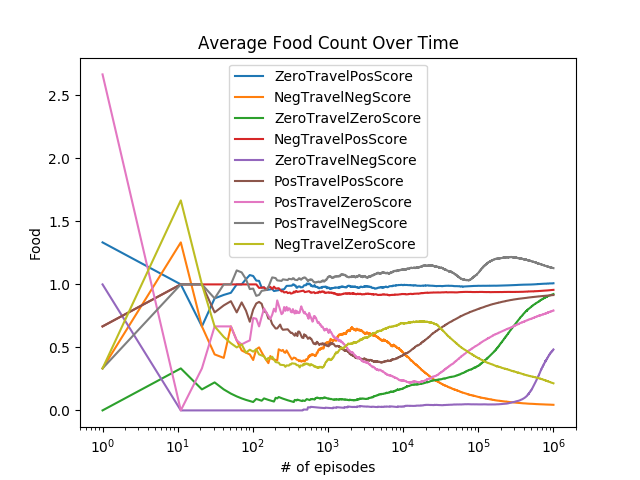
\includegraphics[width=\linewidth]{../images/qlearning/reward/234/board_state_average_food_count_over_time.png}
        \end{subfigure}
        \begin{subfigure}[b]{.35\linewidth}
            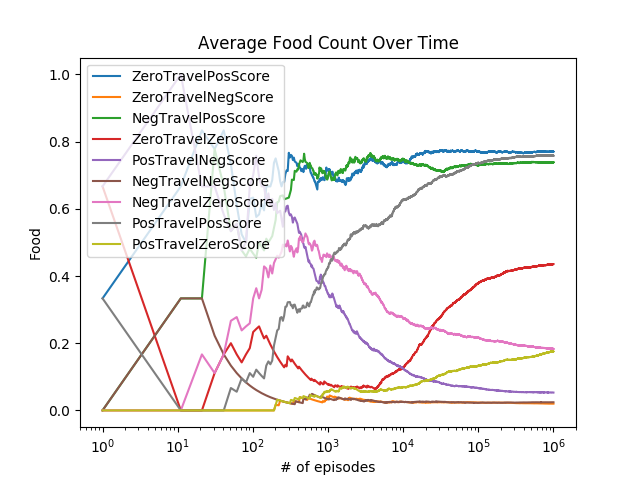
\includegraphics[width=\linewidth]{../images/qlearning/reward/234/directional_distance_state_average_food_count_over_time.png}
        \end{subfigure}

        \begin{subfigure}[b]{.35\linewidth}
            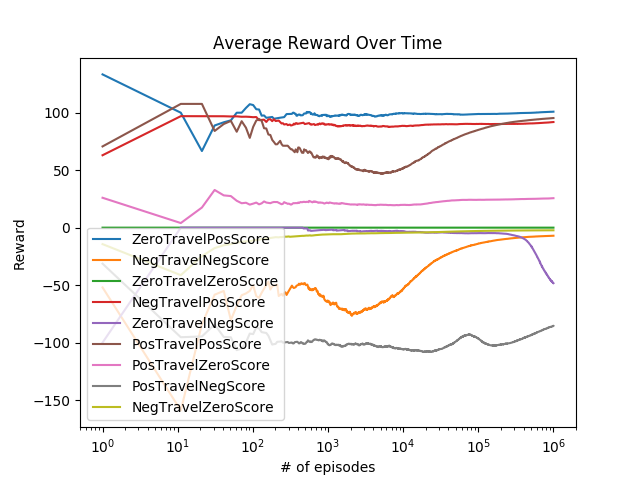
\includegraphics[width=\linewidth]{../images/qlearning/reward/234/board_state_average_reward_over_time.png}
        \end{subfigure}
        \begin{subfigure}[b]{.35\linewidth}
            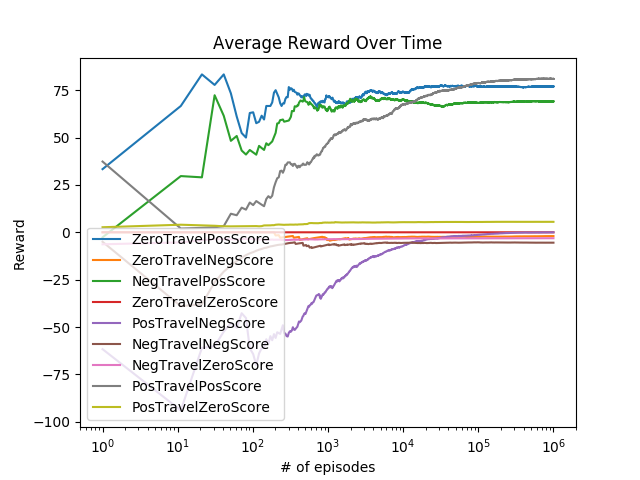
\includegraphics[width=\linewidth]{../images/qlearning/reward/234/directional_distance_state_average_reward_over_time.png}
        \end{subfigure}
        \caption{Results generated by Q-Learning.}
        \label{fig:reward_result_qlearning}
    \end{figure}

    \begin{figure}[ht]
        \centering
        \begin{subfigure}[b]{.35\linewidth}
            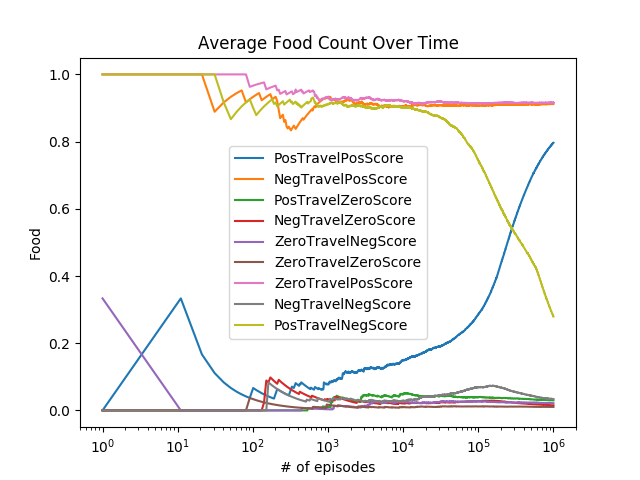
\includegraphics[width=\linewidth]{../images/sarsa/reward/234/board_state_average_food_count_over_time.png}
        \end{subfigure}
        \begin{subfigure}[b]{.35\linewidth}
            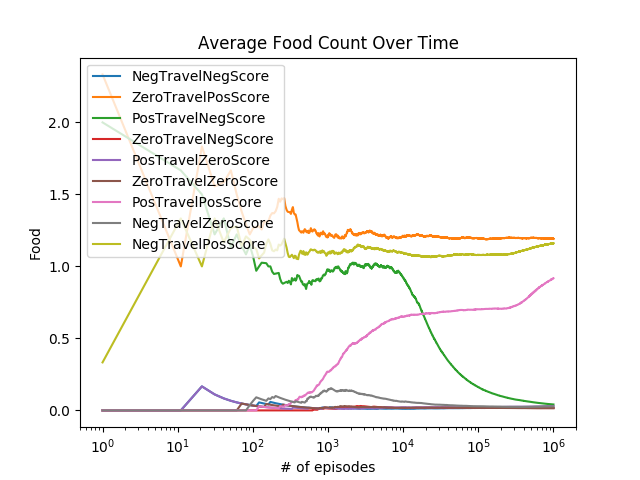
\includegraphics[width=\linewidth]{../images/sarsa/reward/234/directional_distance_state_average_food_count_over_time.png}
        \end{subfigure}

        \begin{subfigure}[b]{.35\linewidth}
            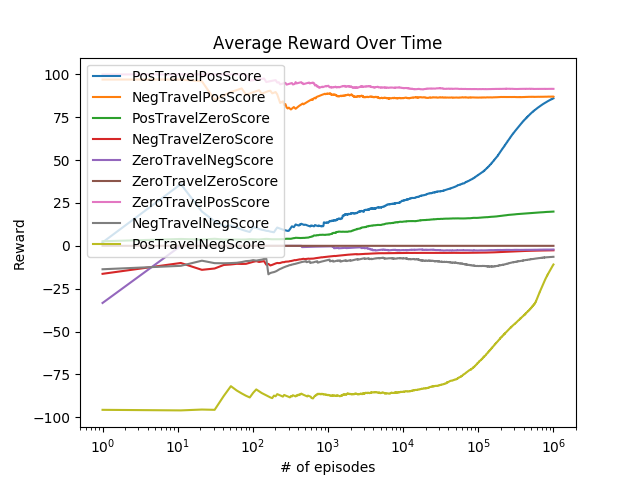
\includegraphics[width=\linewidth]{../images/sarsa/reward/234/board_state_average_reward_over_time.png}
        \end{subfigure}
        \begin{subfigure}[b]{.35\linewidth}
            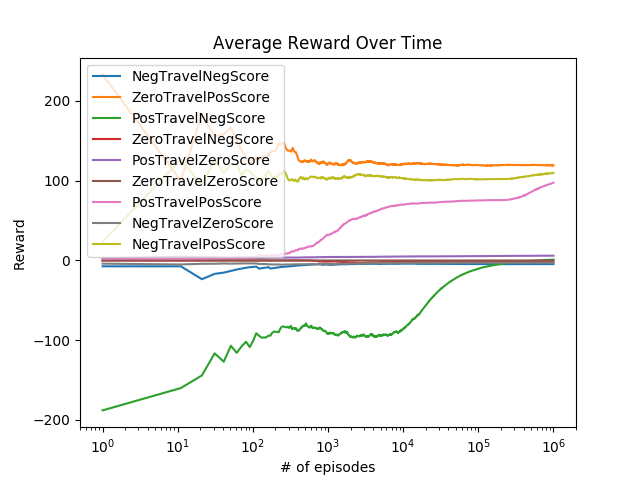
\includegraphics[width=\linewidth]{../images/sarsa/reward/234/directional_distance_state_average_reward_over_time.png}
        \end{subfigure}
        \caption{Results generated by Sarsa.}
        \label{fig:reward_result_sarsa}
    \end{figure}

    \newpage

    \begin{figure}[ht]
        \centering
        \begin{subfigure}[b]{.35\linewidth}
            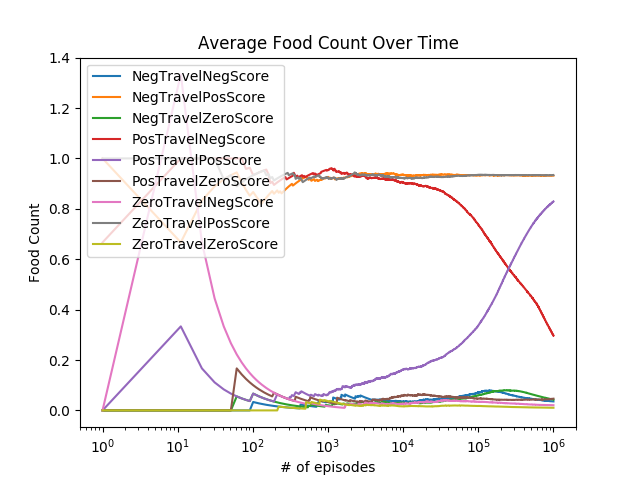
\includegraphics[width=\linewidth]{../images/expected_sarsa/reward/234/board_state_average_food_count_over_time.png}
        \end{subfigure}
        \begin{subfigure}[b]{.35\linewidth}
            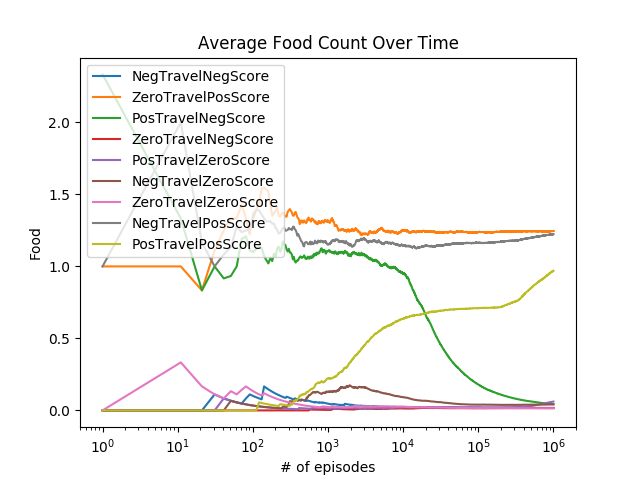
\includegraphics[width=\linewidth]{../images/expected_sarsa/reward/234/directional_distance_state_average_food_count_over_time.png}
        \end{subfigure}

        \begin{subfigure}[b]{.35\linewidth}
            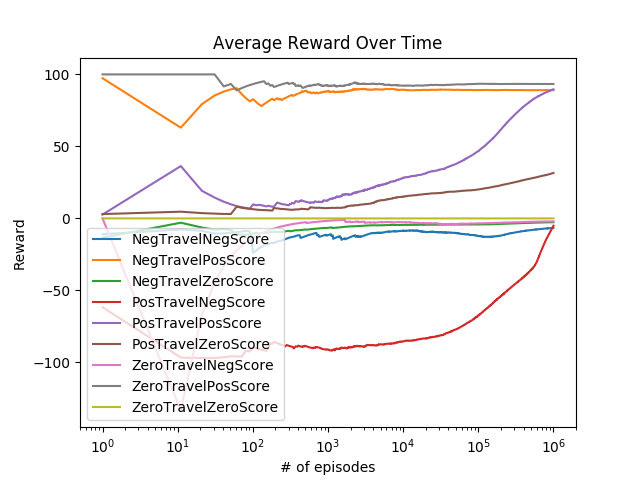
\includegraphics[width=\linewidth]{../images/expected_sarsa/reward/234/board_state_average_reward_over_time.png}
        \end{subfigure}
        \begin{subfigure}[b]{.35\linewidth}
            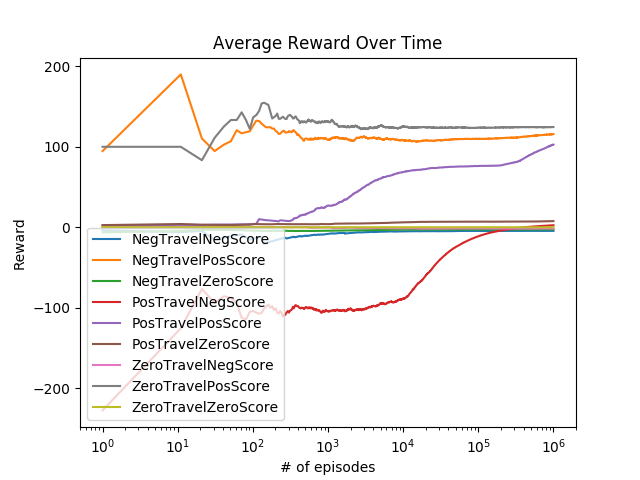
\includegraphics[width=\linewidth]{../images/expected_sarsa/reward/234/directional_distance_state_average_reward_over_time.png}
        \end{subfigure}
        \caption{Results generated by Expected Sarsa.}
        \label{fig:reward_result_expected_sarsa}
    \end{figure}

    The upper plots shows the average food the agent learns to eat on average which is the goal to maximize and the lower plots shows the average reward as a function of time for the different reward functions presented in the method.

    What we mean by \enquote{average over time} is that we take the average of all data points up to (inclusive) the time we are interested in, i.e., a moving average with an infinite tail. In our case time refers to the number of episodes we have trained the model.

    We also looked at the correlation between the curves in the column wise plots above shown in table \ref{tab:reward_food_corr}.

    \begin {table}[H]
        \begin{tabular}{c|c|c|}
            \cline{2-3}
            & \multicolumn{1}{ c| }{Avg. Correlation}
            & \multicolumn{1}{ c| }{Avg. Abs. Correlation} \\
            \cline{2-3}
            & \multicolumn{2}{ c| }{Q-Learning} \\
            \cline{1-3}
            \multicolumn{1}{ |c|  }{Board State}
            & 0.536742184842 & 0.945093533818 \\
            \cline{1-3}
            \multicolumn{1}{ |c|  }{Directional Distance State}
            & 0.49589001223 & 0.973537777401 \\
            \cline{1-3}
            & \multicolumn{2}{ c| }{Sarsa} \\
            \cline{1-3}
            \multicolumn{1}{ |c|  }{Board State}
            & 0.395990504669 & 0.978606301141 \\
            \cline{1-3}
            \multicolumn{1}{ |c|  }{Directional Distance State}
            & 0.521129553421 & 0.963340845075 \\
            \cline{1-3}
            & \multicolumn{2}{ c| }{Expected Sarsa} \\
            \cline{1-3}
            \multicolumn{1}{ |c|  }{Board State}
            & 0.457350122159 & 0.898156494946 \\
            \cline{1-3}
            \multicolumn{1}{ |c|  }{Directional Distance State}
            & 0.507751828694 & 0.968662042717 \\
            \cline{1-3}
        \end{tabular}
        \caption {Correlations between rewards and food counts.}
        \label{tab:reward_food_corr}
    \end{table}

    \newpage

    \subsubsection*{State Experiment}

    In this section we present the results from the state experiment. For each algorithm we have looked at the 16 states presented in the method and they are presented in three plots. Since the goal is to look at the objective of the problem we plot the average food count each state gets over 1 million episodes of training. Same as before we have averaged the result over 3 experiments. Since there is an apparent pattern in the results each result has been divided into 3 plots to emphasize and demonstrate that.

    \begin{figure}[ht]
        \centering
        \begin{subfigure}[b]{.35\linewidth}
            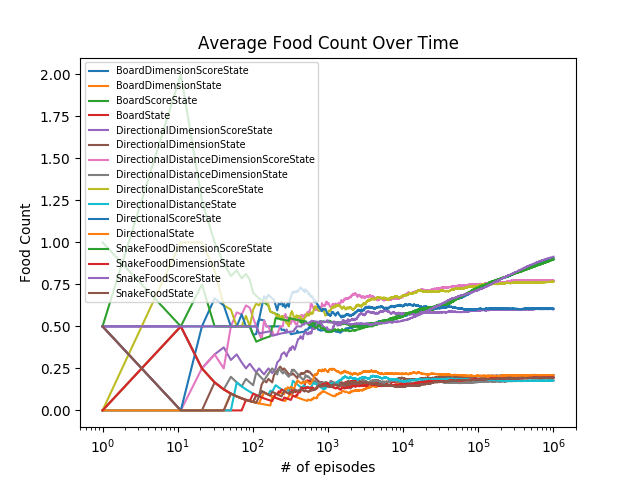
\includegraphics[width=\linewidth]{../images/qlearning/state/234/all_average_food_count_over_time.png}
        \end{subfigure}
        \begin{subfigure}[b]{.35\linewidth}
            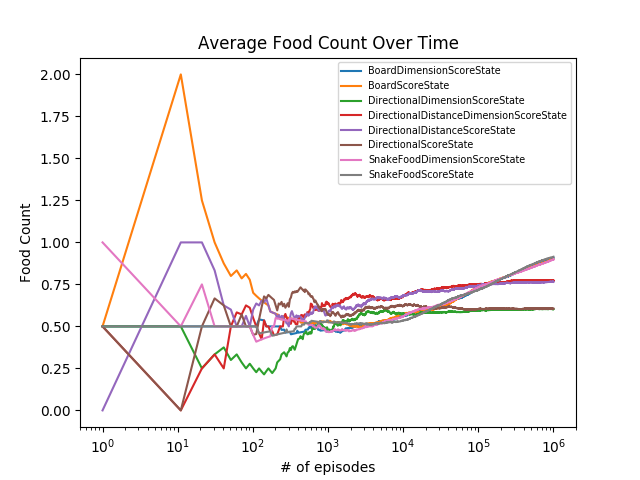
\includegraphics[width=\linewidth]{../images/qlearning/state/234/score_dim_average_food_count_over_time.png}
        \end{subfigure}

        \begin{subfigure}[b]{.35\linewidth}
            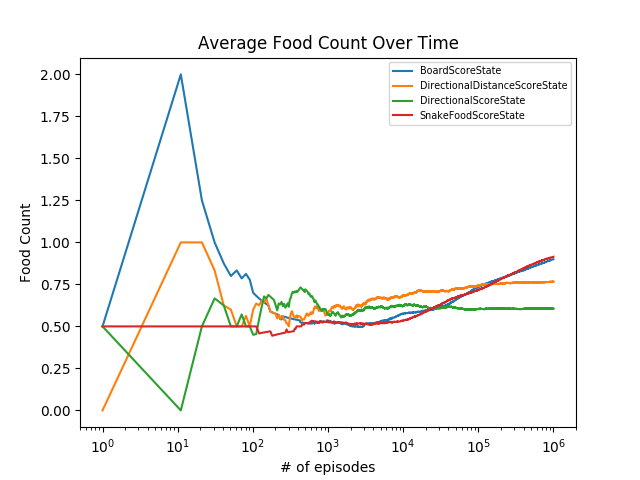
\includegraphics[width=\linewidth]{../images/qlearning/state/234/score_average_food_count_over_time.png}
        \end{subfigure}
        \caption{Results generated by Q-Learning.}
        \label{fig:state_result_qlearning}
    \end{figure}

    \begin{figure}[ht]
        \centering
        \begin{subfigure}[b]{.35\linewidth}
            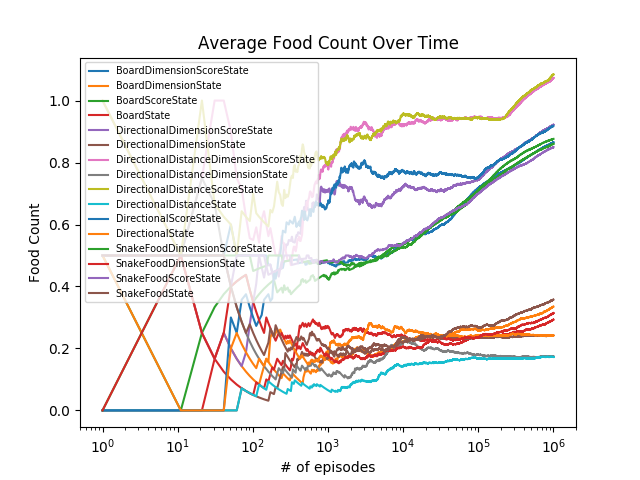
\includegraphics[width=\linewidth]{../images/sarsa/state/234/all_average_food_count_over_time.png}
        \end{subfigure}
        \begin{subfigure}[b]{.35\linewidth}
            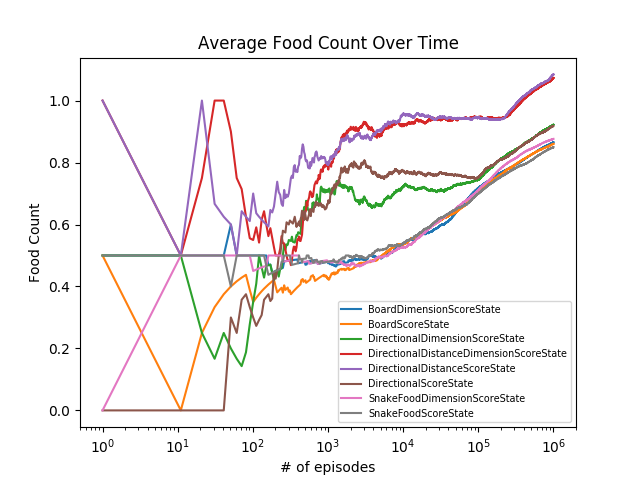
\includegraphics[width=\linewidth]{../images/sarsa/state/234/score_dim_average_food_count_over_time.png}
        \end{subfigure}

        \begin{subfigure}[b]{.35\linewidth}
            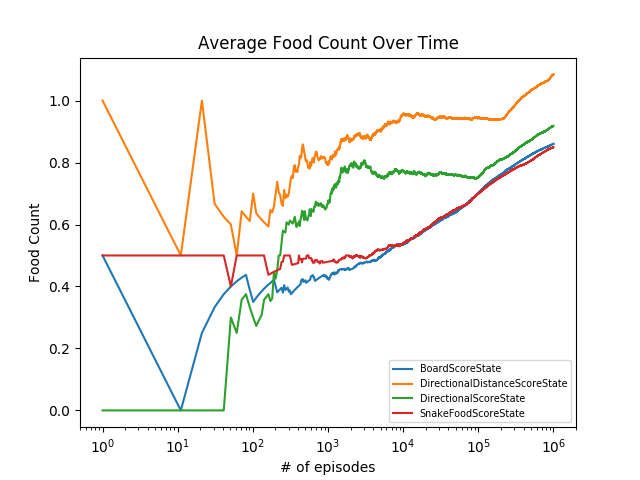
\includegraphics[width=\linewidth]{../images/sarsa/state/234/score_average_food_count_over_time.png}
        \end{subfigure}
        \caption{Results generated by Sarsa.}
        \label{fig:state_result_sarsa}
    \end{figure}

    \newpage

    \begin{figure}[ht]
        \centering
        \begin{subfigure}[b]{.35\linewidth}
            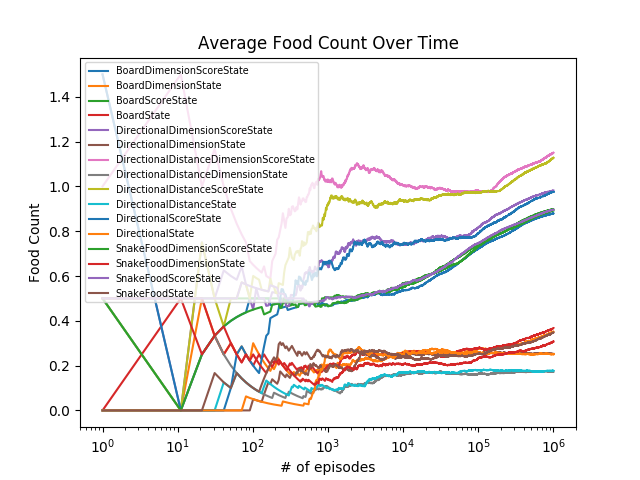
\includegraphics[width=\linewidth]{../images/expected_sarsa/state/234/all_average_food_count_over_time.png}
        \end{subfigure}
        \begin{subfigure}[b]{.35\linewidth}
            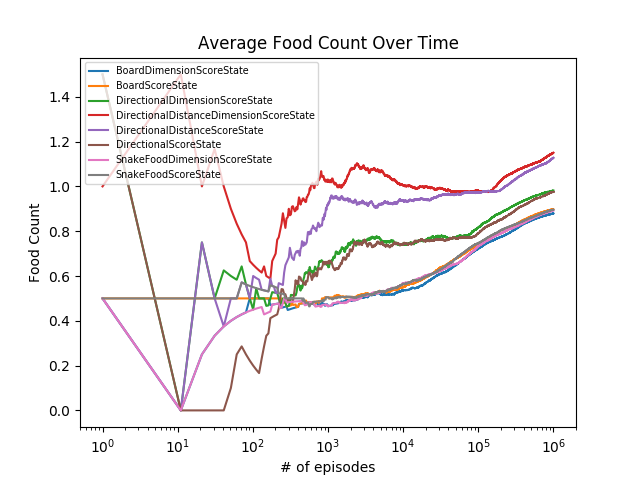
\includegraphics[width=\linewidth]{../images/expected_sarsa/state/234/score_dim_average_food_count_over_time.png}
        \end{subfigure}

        \begin{subfigure}[b]{.35\linewidth}
            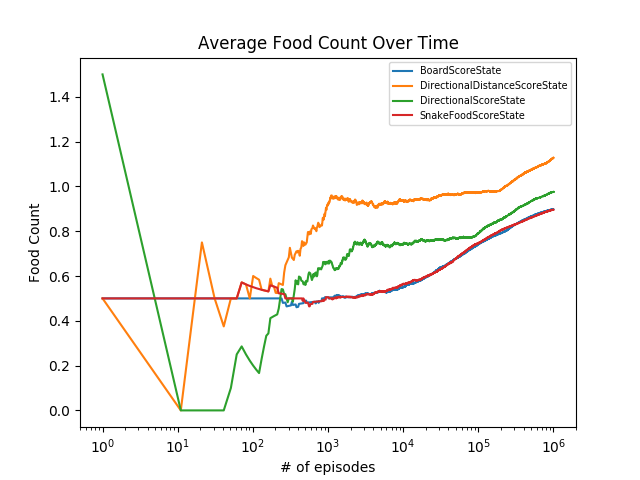
\includegraphics[width=\linewidth]{../images/expected_sarsa/state/234/score_average_food_count_over_time.png}
        \end{subfigure}
        \caption{Results generated by Expected Sarsa.}
        \label{fig:state_result_expected_sarsa}
    \end{figure}

    The 3 plots for each algorithm shows the result for all the states (top-left), the states that contain score information (top-right), and those that contain score information but not board dimensions (bottom-center).

\end{document}
